\documentclass[twocolumn]{ctexart}
% ctexart、ctexrep、ctexbook和ctexbeamer, 对应 LaTeX 的article、report、book和beamer
\usepackage[a4paper,left=3cm,right=3cm,top=2.6cm,bottom=2.6cm]{geometry} % 设置页面尺寸
\usepackage{fancyhdr} % 设置页眉页边页脚
\usepackage{multicol} % 多栏排版
\usepackage{xeCJK} % 中文支持
\usepackage{ctex} % 中文支持
\usepackage{footmisc} % 控制脚注格式,包括编号、字体、分隔线等
\usepackage{titletoc} % 定制目录列表样式
\usepackage{fontspec} % XeTeX下的字体选择宏包
\usepackage{setspace} % 行距
\usepackage{graphicx} % 插图
\usepackage{pdfpages} % 引用pdf页面
\usepackage{booktabs} % 三线表
\usepackage{multirow} % 表格多行支持
\usepackage{caption} % figure和table等中的说明文字
\usepackage{tikz} % 绘图
\usepackage{etoolbox} % 给宏包打补丁
\usepackage{hyperref} % 超链接
\usepackage{xcolor} % 颜色支持
\usepackage{array} % 数学表格
\usepackage{amsmath} % 数学公式
\usepackage{amssymb} % 数学字体与符号
\usepackage{amsthm} % 数学定理格式
\usepackage{subfig} % 排版子图
\usepackage{float} % 浮动体格式控制
\usepackage{lmodern} % 一种字体支持
\usepackage{listings} % 插入代码
\usepackage{tcolorbox} % 好看的块环境
\usepackage{pifont} % 字体支持
\usepackage{perpage} %the perpage package
\usepackage{mathdesign} % some math fonts
\usepackage{ulem} %一些文字强调的宏包
\usepackage{fancyvrb} % some fancy verbatim 
\usepackage{enumitem} % 列表项目
\usepackage{txfonts} % 一些字体
\usepackage{makecell}
\usepackage{mathrsfs}
\usepackage{subfig}                 % 子图包,不要与{subfigure}混用,{subfig}较新
\usepackage{overpic}   
%重置每页脚注序号
\pagestyle{headings}
\MakePerPage{footnote} %the perpage package command
\renewcommand \thefootnote{\ding{\numexpr171+\value{footnote}}}
% 为tcolorbox导入三个程序包
\tcbuselibrary{skins, breakable, theorems} 

% 设置代码格式 - 关键字加粗, 其余为正常。非彩色
\lstset{
    aboveskip=5mm,
    belowskip=5mm,
    breaklines=true,
    breakatwhitespace=true,
    columns=flexible,
    extendedchars=false,
    showstringspaces=false,
    numbers=none,
    basicstyle={\small\ttfamily},
    captionpos=t,
    frame=tb,
    tabsize=4
}

\lstdefinestyle{cpp} {
  language=C++
}

\lstdefinestyle{c++} {
  language=C++
}

\lstdefinestyle{python} {
  language=python,
  morekeywords={as}
}


% 为目录添加 PDF 链接
\addtocontents{toc}{\protect\hypersetup{hidelinks}}

% 设置「目录」二字格式
\renewcommand{\contentsname}{
  \fontsize{16pt}{\baselineskip}
  \normalfont\heiti{目~~~~录}
  \vspace{-8pt}
}

% 定理、定义、证明
\newtheorem{theorem}{定理}[section]
\newtheorem{definition}{定义}[section]
\newtheorem{lemma}{引理}[section]
\newtheorem{corollary}{推论}[section]
\newtheorem{example}{例}
\newtheorem{proposition}{命题}[section]

\title{光学}
\author{洛白}
\date{\today}

\begin{document}

% 显示标题作者时间
\maketitle
\newpage

% 调整目录行间距
\renewcommand{\baselinestretch}{1.35}
% 添加目录
\tableofcontents
\newpage

% 正文 22 磅的行距
\setlength{\parskip}{0em}
\renewcommand{\baselinestretch}{1.53}

\section{球面和球面系统}
可见光是一种波长在380-760$nm$ 波段的电磁波
        \begin{figure}[H]
            \centering
            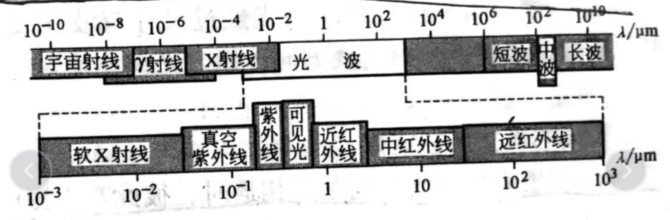
\includegraphics[width=8cm]{img/0.1.png}
            \end{figure}
\begin{quote}
{\qquad\parindent2\ccwd\kaishu\zihao{5}
虚实像物点,物像空间。
}
\end{quote}
\subsection{概念和符号系统}
\subsubsection{完善成像条件}
\begin{enumerate}[nosep]% nosep表示没有垂直间隔
    \item 同心光束成同心光束
    \item 球面波成球面波
    \item 物点像点之间等光程
\end{enumerate}
\subsubsection{一些成像中的概念}
\begin{description}[leftmargin=1.7cm,style=nextline,nosep]% nosep没有垂直间隔
    \item[同心光束] 从同一点发出的或\textbf{汇聚到同一点}的光线束。
    \item[光具组] 若干反射折射面组成的光学系统
    \item[虚实像物点] 同一点发出(实际光线汇聚)的为\textbf{实物}(像)点,汇聚(延长线汇聚)到同一点的为\textbf{虚物}(体)点。
    \item[像物方空间] 实际上,一束光经过一个光学系统,整个空间都是物方空间和像方空间,就是有虚实之分。只不过我们习惯上将像(物)实空间叫做像(物)空间。
    
    同时,符号中不带$'$ 的为物方,带的为像方。如$l,l',n,n',u,u'$。
\end{description}
\subsubsection{一些规定的概念}
\begin{description}[leftmargin=1.7cm,style=nextline,nosep]% nosep没有垂直间隔
    \item[子午平面] 包含光轴的平面
    \item[截距] 物方或像方光线与光轴交点到顶点的距离。
    \item[倾斜角] 物方或像方光线与光轴的夹角。
\end{description}
\subsubsection{约定的符号}
为了表示各种线段量和角度量的属性,我们约定俗成地规定了一些符号。
\begin{description}[leftmargin=1.7cm,style=nextline,nosep]% nosep没有垂直间隔
    \item[传播方向] 物方到像方,并且定义此方向单位向量$\vec{n}$
    \item[沿轴线段] 从折射球面顶点出发到终点(名称左到右),向量为$\vec{r}$,定义其长度为$\vec{r}\cdot \vec{n}$
    \item[垂轴线段] 光轴上正,下负。如果$\vec{n}=(x_0,y_0)$,定义$\vec{n_v}=(-y_0,x_0)$,从折射球面顶点出发到终点(名称左到右),向量为$\vec{r}$,定义其长度为$\vec{r}\cdot \vec{n_v}$
    \item[间隔$d$] 见上。对于一般角度,类比上个方法。
    \item[角度] 从\textbf{光轴到光线到法线}(\textbf{轴线法}),锐角转向,顺正逆负。
    \item[球面半径] 以球面和主光轴的交点为准到球心做向量$\vec{r}$,$r=\vec{r}\cdot \vec{n}$。如右图,其为
    $$
    L_{OC}
    $$
\end{description}

\subsection{基本公式和定理}
$$
n=\frac{c}{v}
$$
\begin{theorem}[费马原理]
光是沿着光程取极值的路径传播的(极大值、极小值或常数)。
\end{theorem}
\begin{theorem}[马吕斯定律]
    光线束在\textbf{各向同性的均匀介质中}传播时,始终保持着与波面的正交性,并且入射波面与出射波面对应点之间的光程均为定值。
\end{theorem}
几何光学有三个基本定律,分别是\textbf{光的直线传播,光的独立传播,光的折反射定律}。
\subsubsection{光的直线传播} 在各向同性的介质中,不遇到波长量级的障碍物时(衍射),光沿直线传播。
\subsubsection{光的独立传播} 不同光源发出的光,在空间某点相遇时,彼此互不影响。(同一单色点光源,干涉)
\subsubsection{光的折反射定律}
\begin{itemize}
\item 全反射是从光密到光疏,入射角大于临界角。
\item 对于反射
$$ n'=-n
$$
\item 对于折射
$$
n\sin I=n'\sin I'
$$
\begin{quote}
{\qquad\parindent2\ccwd\kaishu\zihao{5}
注意$I,I'$ 是入射和出射和法线所成角。
}
\end{quote}
\end{itemize}
\subsection{基本公式推导(单球面折射)}
我们需要根据入射光线给出的条件$r,n,n',L,U$,求出$L',U'$
\begin{figure}[H]
    \centering
    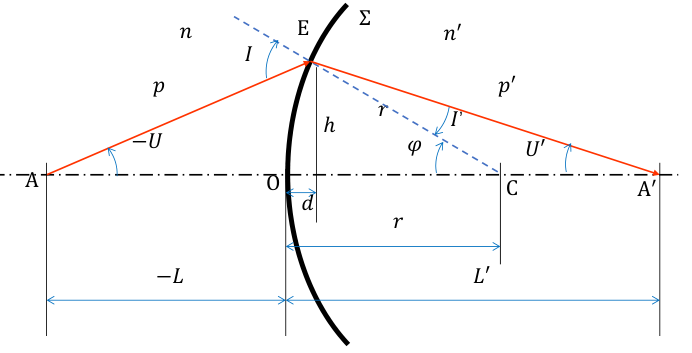
\includegraphics[width=8cm]{img/1.1.png}
\end{figure}
根据折射定律得
\begin{equation}
    n \sin I =n' \sin I '\tag{1.2.1.a}
\end{equation}
在$\Delta EAC$ 中运用正弦定理,得到
\begin{equation}
    \frac{\sin I }{r-L}=\frac{\sin -U}{r}\tag{1.2.2.a}
\end{equation}
显然又因为内外角定理,可得
\begin{equation}
    \varphi=U+I=U'+I' \tag{1.2.3.a}
\end{equation}
在$\Delta ACE$ 中再使用正弦定理,可得
\begin{equation}
    L'=r+\frac{r}{\sin U'} \sin I' \tag{1.2.4.a}
\end{equation}
显然固定$L,r,n,n'$,动$U$,显然$L'$会发生改变,即不是同心光束,
不能\textbf{完善成像}。
\subsubsection{近轴光路近似}

\begin{description}[leftmargin=1cm,style=nextline,nosep]% nosep没有垂直间隔
    \item[近轴(傍轴)光线] 与光轴很靠近的光线,即-U很小,此时\textbf{用小写
            (如-u等)}表示近轴光线的参数。
\end{description}
此时可利用小角近似,$i=\sin i= \tan i$,所以(1.2.1.a-1.2.4.a)可以写成
\begin{align}
    n i =n' i '\tag{1.2.1.b}                 \\
    \frac{i }{r-l}=\frac{-u}{r}\tag{1.2.2.b} \\
    \varphi=u+i=u'+i' \tag{1.2.3.b}          \\
    l'=r+\frac{r}{ u'}  i' \tag{1.2.4.b}
\end{align}
化简(1.2.4.b)
\begin{equation}
    \begin{aligned}
        l'=r+r \frac{i'}{u'} & =r+r \frac{i'}{u+i-i'}                       \\
                             & =r+r \frac{\frac{n}{n'}i}{u+i-\frac{n}{n'}i} \\
                             & =r+r \frac{n}{\frac{n'u}{i}+n'-n}
    \end{aligned}
    \tag{1.2.5}
\end{equation}
先算$i$
\begin{equation}
    i= \frac{u(l-r)}{r}\tag{1.2.6}
\end{equation}
(1.2.6) 代入(1.2.5)
\begin{equation}
    l'=r+r \frac{n}{\frac{n'r}{l-r}+n'-n}\tag{1.2.7}
\end{equation}
显然$l'$与$u$无关,其\textbf{完善成像}。此时的像物点又叫做\textbf{共轭点}。
近轴光所成像称为\textbf{高斯像},
仅考虑近轴光的光学叫\textbf{高斯光学}。
\subsubsection{近轴光路其他公式}
\begin{figure}[H]
    \centering
    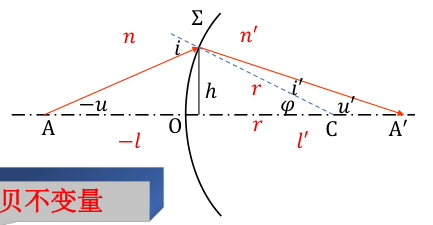
\includegraphics[width=7cm]{img/1.2.png}
\end{figure}
我们新引入了一个$h$,先来引入几个关于它的式子
\begin{align}
    h       & =lu=l'u' \tag{1.2.8}                               \\
    \varphi & \thickapprox \tan \varphi= \frac{h}{r} \tag{1.2.9}
\end{align}
Then Let,s start our solve
\begin{description}[leftmargin=0.7cm,style=nextline,nosep]% nosep没有垂直间隔
    \item[折射球面的物像位置关系]
        由(1.2.8)得,\begin{equation}
            u=\frac{h}{l} \quad u'=\frac{h}{l'} \tag{1.2.10}
        \end{equation}
        化简(1.2.1.b)得{1.2.11.a},其移项化简可得后一项
        \begin{align}
            n(\varphi-u)=n'(\varphi-u') \tag{1.2.11.a} \\
            n u-n' u'=(n-n')\varphi =(n-n')\frac{h}{r} \tag{1.2.11.b}
        \end{align}
        将(1.2.10)代入(1.2.11.b),可得
        \begin{equation}
            \frac{h}{l}n-\frac{h}{l'}n'=(n-n')\frac{h}{r}\tag{1.2.12.bef}\footnote{bef表示该公式的前置证明步骤公式}。
        \end{equation}
        \begin{equation}
            \frac{n}{l}-\frac{n'}{l'}=\frac{n-n'}{r}\tag{1.2.12}
        \end{equation}
        此式即为\textbf{折射球面的物像位置关系},同时,此式也可由式(1.2.7)直接化简而来.下面简要说明
        \begin{equation}
            \begin{aligned}
                l'&=r+r(\frac{n}{\frac{n'r}{l-r}+n'-n})\\
                &=r(1+\frac{nl-nr}{n'r+(n'-n)(l-r)})\\
                &=r(1+\frac{nl-nr}{n'l-nl+nr})\\
                &=r(\frac{n'l}{n'l-nl+nr})
               \end{aligned} \tag{1.2.12.af1}
        \end{equation}
        继续化简
        \begin{align}
         rn'l=(n'&-n)ll'+rnl' \tag{1.2.12.af 2} \\
         r(n'l-nl')&=(n'-n)ll' \tag{1.2.12.af 3}\\
         \frac{n'}{l'}-\frac{n}{l}&=\frac{n'-n}{r} \tag{1.2.12.af 4}   
        \end{align}
        \item[阿贝不变量]
        化简(1.2.11.a)
        \begin{align}
            n(\frac{h}{r}-\frac{h}{l})=n'(\frac{h}{r}-\frac{h}{l'}) \tag{1.2.13.bef} \\
            n(\frac{1}{r}-\frac{1}{l})=n'(\frac{1}{r}-\frac{1}{l'}) =Q \tag{1.2.13}
        \end{align}
        式(1.2.13)即为\textbf{阿贝不变量}公式。
    \item[光焦度]
        表示折射面偏折光线的能力
        \begin{equation}
            \Phi=\frac{n'-n}{r}\tag{1.2.14}
        \end{equation}
    \item[焦距]
        \begin{align}
            \frac{1}{f}=\frac{1}{l_{l' \to \infty}} & =\frac{n-n'}{nr} \tag{1.2.15.a}   \\
            \frac{1}{f'}=\frac{1}{l_{l \to \infty}} & =-\frac{n-n'}{n'r} \tag{1.2.15.b}
        \end{align}
        用光焦度表示的焦距
        \begin{equation}
            \frac{1}{f}= -\frac{1}{n} \Phi\hspace{0.5cm}  \frac{1}{f'}=\frac{1}{n'}\Phi\tag{1.2.16}
        \end{equation}
        化简上述公式可得
        \begin{equation}
            \frac{f'}{f}=-\frac{n'}{n}\tag{1.2.17}
        \end{equation}
        $\displaystyle \frac{1}{(1.2.15.a)}+\frac{1}{(1.2.15.b)}$可得
        \begin{equation}
            f+f'=\frac{1}{r}\tag{1.2.18}
        \end{equation}
        如果对于空气中(理想光学系统),$n=1$就有
        \begin{align}
                f+f'&=\frac{1}{r}=0\tag{1.2.18.a}\\
                \Phi&=-\frac{1}{f}=\frac{1}{f'}\tag{1.2.16.a}
        \end{align}

    \item[屈光度]
        光焦度的单位称为\textbf{屈光度},以字母D表示(对应焦距单位:米)
        \begin{enumerate}[nosep]% nosep表示没有垂直间隔
            \item  200度近视镜光焦度-2.00D(凹透镜)\textcolor{red}{\textbf{负透镜}}
            \item 300度老花镜光焦度3.00D(凸透镜)\textcolor{red}{\textbf{正透镜}}
        \end{enumerate}
    \item[高斯公式]
        将(1.2.15.a),(1.2.15.b)代入式(1.2.12)得
        \begin{equation}
            \frac{n-n'}{r}=\frac{(n-n')f}{rl}+\frac{(n-n')f'}{rl'}  \tag{1.2.19.bre1}
        \end{equation}
        显然可得
        \begin{equation}
            \frac{f}{l}+\frac{f'}{l'}=1 \tag{1.2.19}
        \end{equation}
        式(1.2.19)即为\textbf{高斯公式}。

    \item[牛顿公式]
    设A为物垂点,$A'$为像点垂点,$\displaystyle x=l_{FA},x'=l_{F'A'}$(见下图1.1),有
  \begin{align}
 l&=x+f \tag{1.ad.1.a} \\
 l'&=x'+f' \tag{1.ad.1.b}
  \end{align}
将(1.ad.1.a),(1.ad.1.b)代入式(1.2.19)得
\begin{align}
    \frac{f}{x+f}&+\frac{f'}{x'+f'}=1 \tag{1.ad.2.bef.1} \\
    x'f+2ff'+xf'&=xx'+ff'+x'f+xf' \tag{1.ad.2.bef.2}\\
    ff'&=xx' \tag{1.ad.2}
\end{align}
    % \item[]
\end{description}
\subsubsection{三种放大率和拉氏不变量}
        \begin{figure}[H]
            \centering
            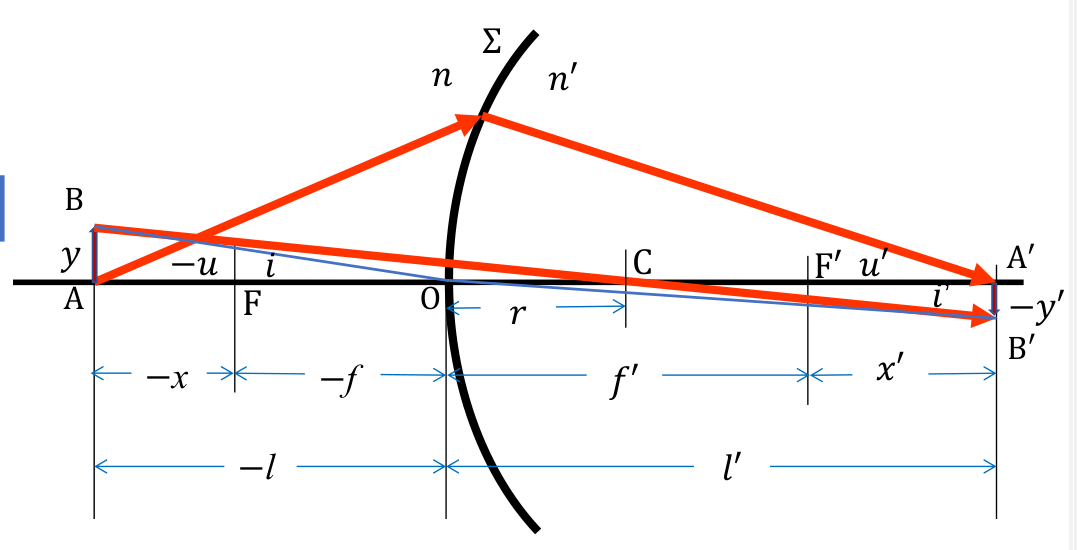
\includegraphics[width=8cm]{img/1.3.png}
            \caption[图1.1]{光路示意图}
            \end{figure}
% 上图中存在错误,我们将图中的$-l$ 记作$l$,$-y'$ 记作$y'$ 注意其均\textbf{带有正负}.
\begin{description}[leftmargin=0.7cm,style=nextline,nosep]% nosep没有垂直间隔
    \item[横向放大率] 
     \begin{equation}
     \beta=\frac{y'}{y}=\frac{l'i'}{li}\tag{1.2.20}
     \end{equation}
     又因为有
\begin{align}
    ni=ni' \quad lu=l'u' \tag{1.2.21.bre 1}\\
        nlui=n'l'u'i'  \tag{1.2.21.bre 2}
\end{align}
所以可得
\begin{equation}
\beta=\frac{nu}{n'u'}=\frac{nl'}{n'l} \tag{1.2.21}
\end{equation}
继续化简
\begin{equation}
\begin{aligned}
    \beta=-\frac{fl'}{f'l}&=-\frac{f(x'+f')}{f'(x+f)}
    \\
    &=-\frac{fx'+xx'}{f'(x+f)}=-\frac{x'}{f'}\\
    &=-\frac{f(x'+f')}{f'x+xx'}=-\frac{f}{x}
\end{aligned}
\tag{1.ad.3}
\end{equation}
\begin{quote}
{\parindent2\ccwd\kaishu\zihao{5}
$\beta>0$正立虚实相反像,$\beta<0$倒立虚实相同像。>1放大,<1缩小。
}
\end{quote}
    \item[横向(垂轴)放大率] 
    \begin{equation}
    \alpha=\frac{\mathrm{d}{ l'}}{\mathrm{d}{l}} \tag{1.2.22.a}
    \end{equation}
    (1.2.12)两端分别对$u$进行求导,r对u是常数,所以有
    \begin{align}
      \frac{n'}{l'^2}\frac{\mathrm{d}{l'}}{\mathrm{d}{u}}-\frac{n}{l^2}\frac{\mathrm{d}{l}}{\mathrm{d}{u}}=0 \tag{1.2.22.bef 1}\\ 
      \frac{n'}{l'^2}\frac{\mathrm{d}{l'}}{1}=\frac{n}{l^2}\frac{\mathrm{d}{l}}{1}\tag{1.2.22.bef 1}
    \end{align}
    所以求得
    \begin{equation}
    \alpha=\frac{\mathrm{d}{l'}}{\mathrm{d}{l}}=\frac{nl'^2}{n'l^2}=\frac{\beta^2}{\frac{n}{n'}}=\frac{n'}{n}\beta^2 \tag{1.2.22}
    \end{equation}

    % 或者有一种更为简单的推导方法,使用(1.ad.2),可得
    \item[角放大率]
    \begin{equation}
    \gamma=\frac{u'}{u}=\frac{l}{l'}=\frac{1}{\beta}\frac{n}{n'} \tag{1.2.23}
    \end{equation} 
    或者说
    \begin{equation}
    \beta=\frac{nu}{n'u'}=\frac{n}{n'} \frac{1}{\gamma} \tag{1.add.4}
    \end{equation}
\end{description}
显然以上三种放大率$\alpha \hspace{0.2cm}  \beta\hspace{0.2cm}   \gamma$之间存在关系,
\begin{equation}
\alpha\gamma=\beta\tag{1.2.24}
\end{equation}
\begin{description}[leftmargin=0.7cm,style=nextline,nosep]% nosep没有垂直间隔
    \item[拉式不变量] 同时根据$\beta$我们定义一个叫做拉式不变量的概念
    \begin{align}
    \frac{y'}{y}=\beta=\frac{nu}{n'u'}    \tag{1.2.25.bef 1}\\
      nuy=n'u'y'=j  \tag{1.2.25}
    \end{align}
    j为拉氏不变量,它是表征光学系统性能的重要参数
\end{description}

\subsection{反射球面}\
其实就是将$n+n'=0$代入上述所有基本公式进行化简,下面给出部分常用公式
\begin{align}
\Phi&=\frac{-2n}{r}=\frac{2n'}{r} \tag{1.2.26} \\
f&=f'=\frac{r}{2} \tag{1.2.27} \\
&\frac{1}{l}+\frac{1}{l'}=\frac{2}{r} \tag{1.2.28}
\end{align}
% \subsection{共轴球面系统}
% \subsection{透镜}
\section{薄透镜理想光学系统}
\subsection{共轴球面系统}
\begin{figure}[H]
    \centering
    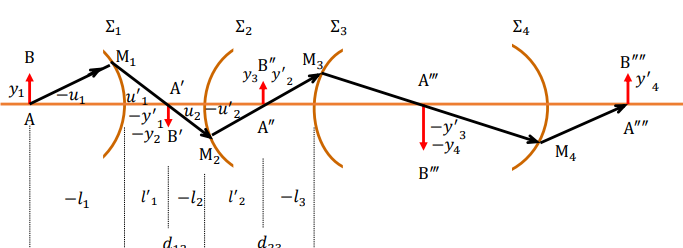
\includegraphics[width=8cm]{img/1.4.png}
    \end{figure}
    \subsubsection{过渡公式}
第$i$面的物方空间就是第$i+1$面的像方空间。所以
\begin{align}
    n_{i+1}&=n'_{i} \tag{2.add.1.a}\\
     u_{i+1}&=u'_{i} \tag{2.add.1.b}\\
     y_{i+1}&=y'_{i} \tag{2.add.1.c} 
\end{align}
同时有
\begin{align}
d_i=d_{i(i+1)}&=l_{i}'-l_{i+1} \tag{2.add.2.pre} \\
l_{i+1}&=l_{i}'-d_i \tag{2.add.2}
\end{align}
(2.add.2)乘(2.add.1.b)可得($h_i=l_iu_i$)
\begin{equation}
h_{i+1}=h_i-d_i u_{i}'\tag{2.add.3}
\end{equation}
对每个面应用拉式不变量和过度公式(2.add.1)可得
\begin{align}
    n_iu_iy_i=J \tag{2.add.4}
\end{align}
       
\subsubsection{放大率}
\begin{align}
    \alpha_n=\frac{\mathrm{d}{l'_n}}{\mathrm{d}{l_1}}=\prod_{i=1}^n \alpha_i \tag{2.1.1.a}\\
    \beta_n=\frac{y_n'}{y_1}=\prod_{i=1}^n \beta_i \tag{2.1.1.b}\\
    \gamma_n=\frac{u_n'}{u_1}=\prod_{i=1}^n \gamma_i \tag{2.1.1.c}
\end{align}
其关系顺延之前。
\subsection{薄透镜}
\begin{description}[leftmargin=0.7cm,style=nextline,nosep]% nosep没有垂直间隔
    \item[薄透镜] 透镜厚度d 远小于物距、像距、焦距、曲率半径等 
       \begin{figure}[H]
                \centering
                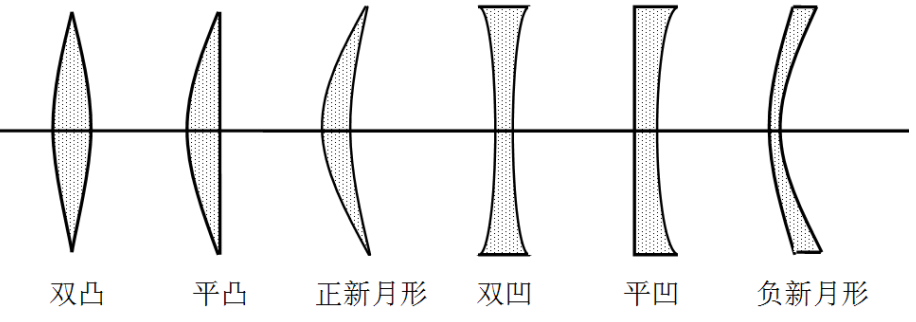
\includegraphics[width=8cm]{img/1.5.png}
                \end{figure}
\end{description}
\subsubsection{成像}        \begin{figure}[H]
            \centering
            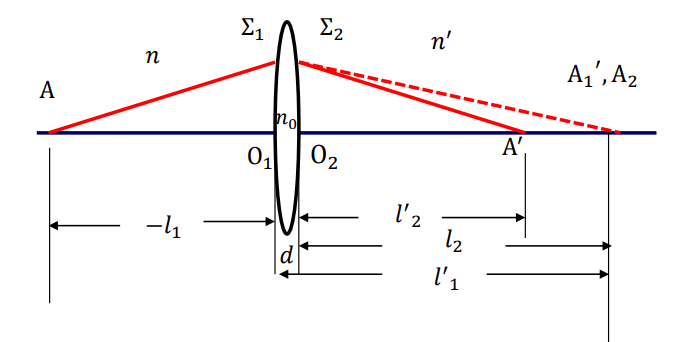
\includegraphics[width=8cm]{img/1.7.png}
            \end{figure}
\begin{align}
    \frac{n_0}{l_1'}-\frac{n}{l_1}=\frac{n_0-n}{r_1} \tag{2.2.1.a}\\
    \frac{n'}{l_2'}-\frac{n_0}{l_2}=\frac{n'-n_0}{r_2} \tag{2.2.1.b}
\end{align}
并且
\begin{equation}
l_2=l_1'+d \thickapprox  l_1' \tag{2.2.2}
\end{equation}
(2.2.1.a)+(2.2.1.b)
\begin{align}
    \frac{n'}{l_2'}-\frac{n}{l_1}=\frac{n_0-n}{r_1}+\frac{n'-n_0}{r_2}\tag{2.2.3.a}\\
    \frac{n'}{l'}-\frac{n}{l_1}=\frac{n_0-n}{r_1}+\frac{n'-n_0}{r_2}\tag{2.2.3.b}
\end{align}
(2.2.3.b) 就是\textbf{薄透镜傍轴成像的物像距公式}。化简一下
\begin{equation}
    n(\frac{1}{r_1}-\frac{1}{l})-n'(\frac{1}{r_2}-\frac{1}{l'})=n_0(\frac{1}{r_1}-\frac{1}{r_2}) \tag{2.2.4}
\end{equation}
设(2.2.3.b)等式右边为$\Phi$,可得
\begin{align}
\text{物方焦距}f=\lim_{l' \to \infty}\frac{-n}{\Phi} \tag{2.2.5.a}\\
\text{像方焦距}f'=\lim_{l \to \infty}\frac{n'}{\Phi} \tag{2.2.5.b}\\
f=-f'=\frac{n}{\Phi} \tag{2.2.5.c}
\end{align}
$f'>0$汇聚$<0$发散。联立以上各方程组,可得其牛顿公式和高斯公式基本不变
\begin{align}
    \text{高斯公式}\frac{f'}{l'}+\frac{f}{l}=1 \tag{2.2.6.a}\\
    \text{牛顿公式}xx'=ff' \tag{2.2.6.b}
\end{align}

并且如果在空气中$n=n'=1$,可得
\begin{align}
f'=-f=\frac{1}{\Phi} \tag{2.2.7.a}\\
\Phi=(n_0-1)(\frac{1}{r_1}-\frac{1}{r_2}) \tag{2.2.7.b}
\end{align}
$\displaystyle \Phi>0,\frac{1}{r_1}-\frac{1}{r_2}>0$ 凸透镜,反之凹透镜。(其实只考虑两种最极端的情况就行)
对于放大率来说,
\begin{align}
 \beta_1=\frac{n_1l_1'}{n_1'l_1} \tag{2.2.8.a}\\
 \beta_2=\frac{n_2l_2'}{n_2'l_2} \tag{2.2.8.b}\\
 \beta=\beta_1 \beta_2=\frac{n_1n_2l_1'l_2'}{n_1'n_2'l_1l_2} \tag{2.2.8.c}\\
 l_1'=l_2,l_1=l,l_2'=l'\tag{2.2.8.d}\\
 n_1=n,n_2'=n',n_1'=n_2=n_0\tag{2.2.8.e}
\end{align}
联立以上五式可得
\begin{equation}
\beta=\frac{nl'}{n'l}=-\frac{fl'}{f'l} \tag{2.2.9}
\end{equation}
注意上式中$f,f'$的顺序
$$
fn'+f'n=0
$$
下面再来看几个放大率,一样的分析方法(略去一点推导)
        \begin{figure}[H]
            \centering
            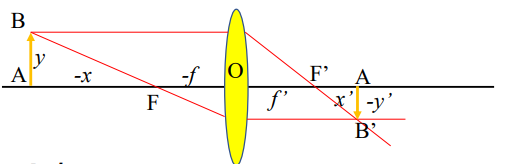
\includegraphics[width=8cm]{img/1.8.png}
            \end{figure}
            \begin{align}
                -\frac{y'}{y}=\frac{f}{x}=\frac{x'}{f'} \tag{2.2.10.a}\\
                \beta=\frac{y'}{y}=-\frac{f}{x}=-\frac{x'}{f'} \tag{2.2.10.b}
            \end{align}
            然后一如既往的
            \begin{align}
                \alpha=\frac{n'}{n}\beta^2 \tag{2.2.11.a}\\
                \gamma=\frac{n}{n'}\frac{1}{\beta}\tag{2.2.11.b}\\
                \alpha \gamma=\beta \tag{2.2.11.c}
            \end{align}
\textcolor{red}{\textbf{注意算透镜的时候,多用焦距,这样十分简单。}}
        \begin{figure}[H]
            \centering
            
\includegraphics[width=8cm]{img/1.9.png}
            
\includegraphics[width=8cm]{img/1.10.png}

            \end{figure}
\section{理想光学系统}
单个折射球面或者是单薄透镜是对细小平面以细光束成完善像,但是实际的光学系统
需要对一定大小的场以宽光束成像,其\textbf{成像有缺陷}。所以其必须要由若干元件组成,经过反复计算,使其成像\textbf{趋于}完善。

并且对于理想光学系统,所成的像是完全相似的。这种理想光学系统理论,也被称作\textbf{高斯光学}。并且引出共轭的表示
\begin{align}
    \text{点} \to \text{共轭点} \tag{3.0.a}\\
    \text{线} \to \text{共轭线} \tag{3.0.b}\\
    \text{面} \to \text{共轭面} \tag{3.0.c}\\
    \text{同心光束} \to \text{共轭同心光束} \tag{3.0.d}
\end{align}
\subsection{共线成像理论}
由于系统的对称性,理想共轴光学系统有如下性质
\begin{description}[leftmargin=1.7cm,style=nextline,nosep]% nosep没有垂直间隔
    \item[光轴] 光轴物点的共轭点还在光轴上
    \item[子午平面] 通过光轴的平面,物点的共轭点在一子午平面上
    \item[垂轴平面] 物面垂轴,其共轭像面一定也垂轴,并且几何形状相似。
    \item[表示] 如果已知两对共轭平面的位置和$\beta$,或者一对共轭平面的位置和$\beta$,以及一对共轭点,则一切物点的像点均可确定。    
    \item[同心] 同心光束还是同心光束(理想成像) 
\end{description}
        \begin{figure}[H]
            \centering
            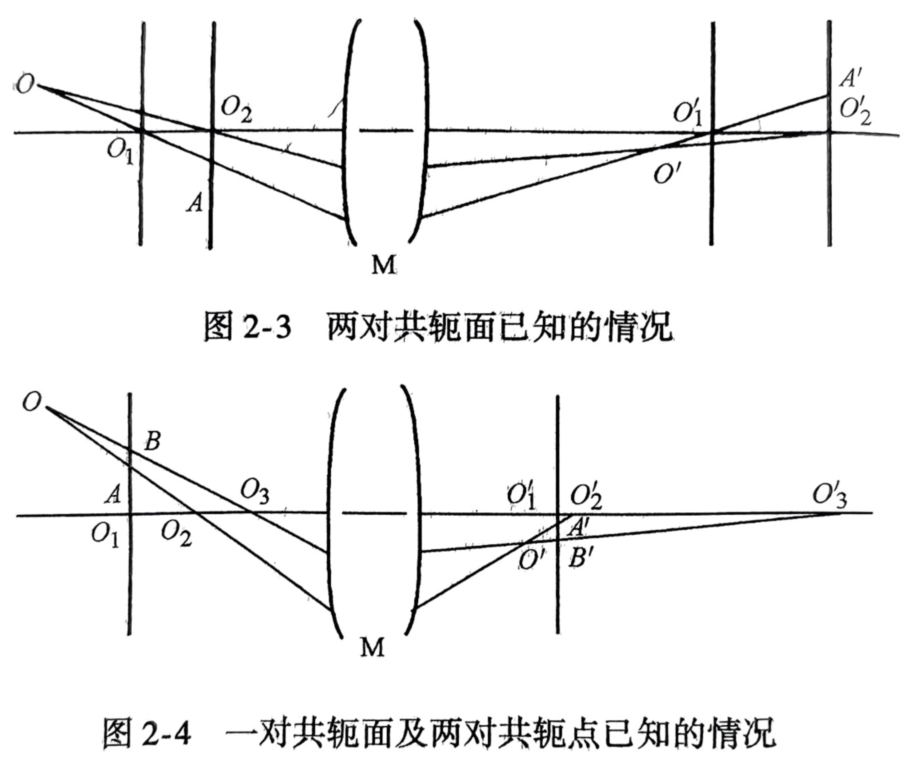
\includegraphics[width=6cm]{img/2.1.png}
            \end{figure}
\subsection{各种定义}

\subsubsection{对于无限物点}
无限远\textbf{轴上}物点发出的同心光束等效于平行于光轴的平行光束,其共轭像点为$F'$。对于轴外的话,就是下图所示
        \begin{figure}[H]
            \centering
            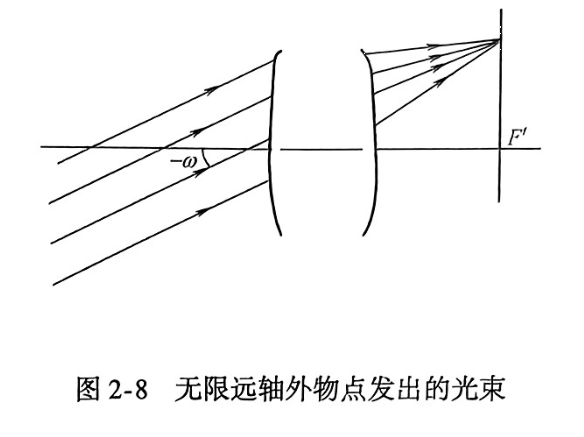
\includegraphics[width=7cm]{img/3.10.png}
            \end{figure}
\subsubsection{对于无限像点}
同上
\subsubsection{焦点和焦面}
        \begin{figure}[H]
            \centering
            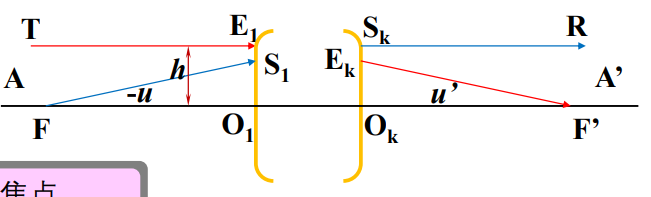
\includegraphics[width=8cm]{img/1.11.png}
            \end{figure}
            对于无穷远轴上像物点$A',A$

            \begin{align}
        A \to F' \tag{3.2.1.a} \\
        F \to A' \tag{3.2.1.b} 
    \end{align}
    物方无穷远垂轴平面的共轭平面为通过 F’的垂轴平面(后焦平面,像方焦面),像方无穷远垂轴平面的共轭平面为物方过 F 的垂轴平面(前焦平面,物方焦面)。
\begin{quote}
{\parindent2\ccwd\kaishu\zihao{5}
物方无穷远垂轴平面一轴外点,其所成平行光一定交于后焦平面一点。显然此两平面共轭。像方同理。
}
\end{quote}
\begin{align}
f=\frac{h}{\tan U} \tag{3.2.2.a}\\
f=\frac{h}{\tan U'} \tag{3.2.2.b}
\end{align}
\footnote[1]{这时候用大写的,因为有轴外物点,其不再满足前文所述\textbf{傍轴条件}}
    \subsubsection{主点$H,H'$和主平面}
    \begin{definition}[主平面]
    $\beta=1$ 的一对平面
    \end{definition}
    \begin{figure}[H]
        \centering
        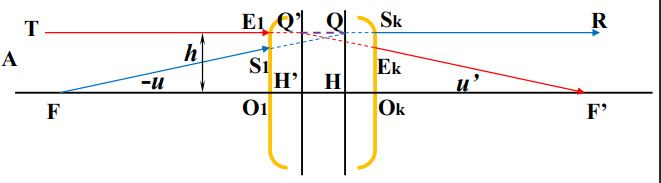
\includegraphics[width=7cm]{img/3.1.png}
        \end{figure} 
如图所示找到$Q,Q',H,H'$
\begin{align}
    Q \to Q' \tag{3.2.3.a}\\
    H \to H' \tag{3.2.3.b}\\
    QH \to QH' \quad (\beta=1) \tag{3.2.3.c}\end{align}
\begin{quote}
{\parindent2\ccwd\kaishu\zihao{5}
主点H,带不带'取决于其经过是像方焦点还是物方焦点。显然对于正透镜,左边是$H'$,对于负透镜,$f'< 0$,左边是$H$

}
\end{quote}
% \subsubsection{焦距}
% \begin{align}
% f'=\overline{H'F'}=\frac{h}{u'} \tag{2.3.3.a}\\
% f=\overline{HF}=\frac{h}{u} \tag{2.3.3.b}
% \end{align}
\subsubsection{基点}
无限远轴外像物点$A,A'$,和像方、物方焦点$F,F'$以及主面的交点$H,H'$,可以确定所有物点的像点,代表一个理想光学系统。

同时对于一些特殊的折射球面,单个折射球面,球面镜和波透镜都相当于两个主面重叠的情况。
\begin{quote}
{\parindent2\ccwd\kaishu\zihao{5}
$H,H',F,F'$这四点就称作光学系统的\textbf{基点}。
}
\end{quote}
\subsubsection{节点$J,J'$}
一对$\gamma=1$的共轭点。物方入射于 J 的任意光线,将以相同方向从 J’射出
        \begin{figure}[H]
            \centering
            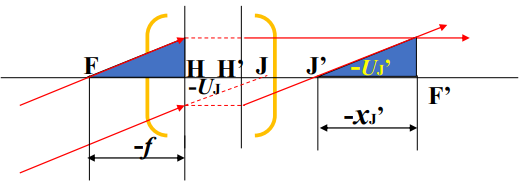
\includegraphics[width=8cm]{img/3.2.png}
            \end{figure}
由三角形全等,显然可得
\begin{align}
    x_J'={F'J'}=f \tag{3.2.4.a} \\
    X_J=FJ=f' \tag{3.2.4.b}
 \end{align}
当$f=f'$有
\begin{align}
    x_J'={F'J'}=-f'=F'H' \tag{3.2.4.a} \\
    X_J=FJ=f'=-f=FH \tag{3.2.4.b}
 \end{align}

节点$J,J'$和主点$H,H'$重合,这时光学系统两边折射率相同。

\subsubsection{各物理量的表示}
        \begin{figure}[H]
            \centering
            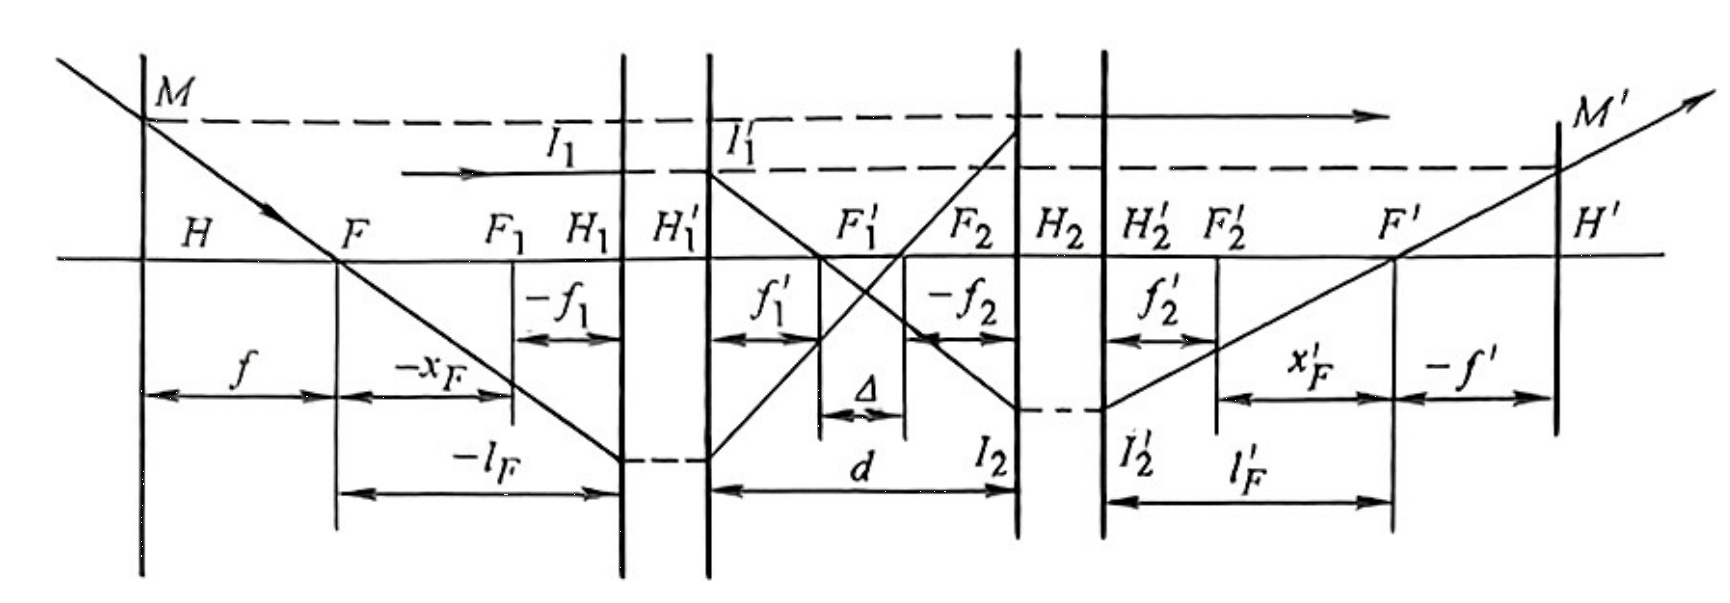
\includegraphics[width=9cm]{img/3.12.png}
            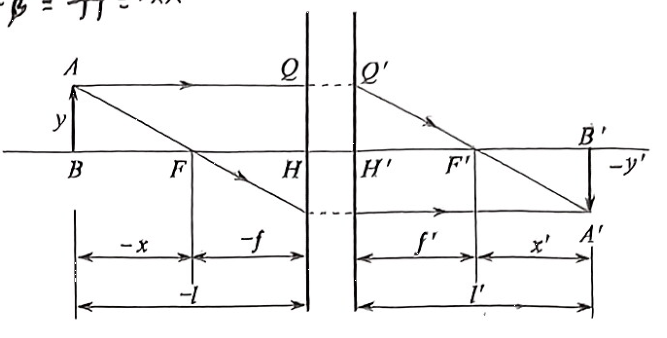
\includegraphics[width=6cm]{img/3.13.png}
            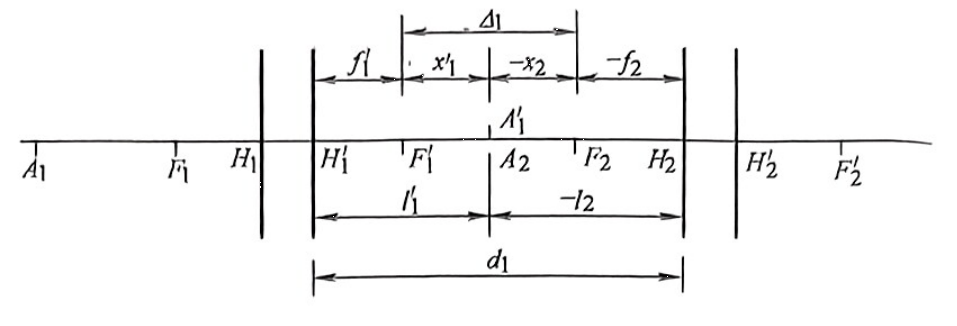
\includegraphics[width=8cm]{img/3.14.png}
            \caption[图2.1]{两光组组合及符号示意图}
            \end{figure}
如上图2所示,有
\begin{align}
 f_{i}=H_{i}F_{i} \quad& f'_{i}=H'_{i}F'_{i} \tag{3.2.5.a}\\
 x_{i}=F_{i}A_{i} \quad& x'_{i}=F'_{i}A'_{i} \tag{3.2.5.b}\\
 l_i=H_iA_i \quad& l'_i=H'_iA'_i \tag{3.2.5.c}\\
 A_i'=A_{i+1}& \tag{3.2.5.d}\\
 d_i=H_{i}'H_{i+1} &=l_{i}'-l_{i+1}\tag{3.2.5.e}\\
 \Delta_i=F_{i}'F_{i+1}&=x_i'-x_{i+1} \tag{3.2.5.f}\\
 l_{F}=H_1 F \quad & l_{F}'=H_2' F' \tag{3.2.5.g}\\
 l_{H}=H_1 H \quad & l_{H}'=H_2' H' \tag{3.2.5.h}
\end{align}
显然通过对以上公式的化简,有
    \begin{align}
        \Delta_i=F_{i}'F_{i+1}=-f_i'+d_{i}+f_{i+1} \tag{3.2.6.a}
    \end{align}
\subsection{理想光学系统的物像位置关系和放大率}
        \begin{figure}[H]
            \centering
            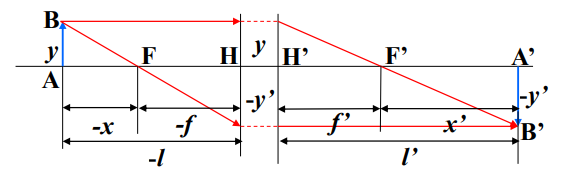
\includegraphics[width=8cm]{img/3.3.png}
            \end{figure}
看图显然可以得到
\begin{equation}
\beta=\frac{y'}{y}=-\frac{x'}{f'}=-\frac{f}{x}\tag{2.3.5}
\end{equation}
% 最显然的我们可以得到
% \begin{align}
%     x x'=f f' \tag{2.3.5.a}\\
%     \frac{f'}{l'}+\frac{f}{l}=1 \tag{2.3.5.b}\\
%     l=x+f \quad l'=x'+f' \tag{2.3.5.c} \\
%     f'n+fn'=0 \tag{2.3.5.d} \\
%     \beta=\frac{nl'}{n'l}=-\frac{fl'}{f'l} \tag{2.3.5.e}
%     % \frac{n'}{f'}-\frac{n}{f}=\Phi=\frac{n'}{f'}=\frac{-n}{f} \tag{2.3.5.f}
% \end{align}
\begin{quote}
{\parindent2\ccwd\kaishu\zihao{5}
这里只列举一部分,就和第一章一样,参照第一章就好。
}
\end{quote}
如果含有k个反射面,有
\begin{equation}
    \beta=\frac{y'}{y}=(-1)^{k+1}\frac{n'}{n} \tag{2.3.6}
\end{equation}

轴向点移动$\Delta$距离后,其垂轴放大率为
\begin{equation}
\overline{\alpha}=\frac{n'}{n}\beta_1\beta_2 \tag{2.3.7}
\end{equation}
% 将式(2.4.1.c)代入(2.4.1.a)可得(2.4.1.b)
\subsubsection{作图原则}
\begin{description}[leftmargin=1.7cm,style=nextline,nosep]% nosep没有垂直间隔
    \item[同心光束] 同心光束还成同心光束
    \item[轴上] 轴上物点的像点还在轴上  
    \item[主面] $\beta=1$
    \item[节点]  $\gamma =1$
    \item[无穷远像物方轴上点] 平行轴向光,与焦点共轭
    \item[无穷远像物轴外电点] 斜向平行光,与焦面某点共轭   
\end{description}
\begin{quote}
{\qquad\parindent2\ccwd\kaishu\zihao{5}
对于轴外一点,一平行一过焦点。对于轴上,找过A点和F的平行光线或者同心光束,使用以上方法即可。
}
\end{quote}
        \begin{figure}[H]
            \centering
            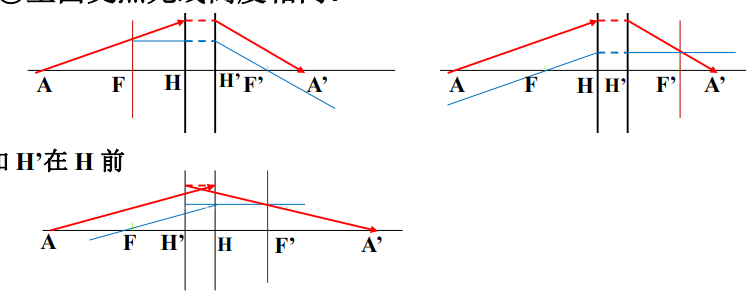
\includegraphics[width=8cm]{img/3.4.png}
            
            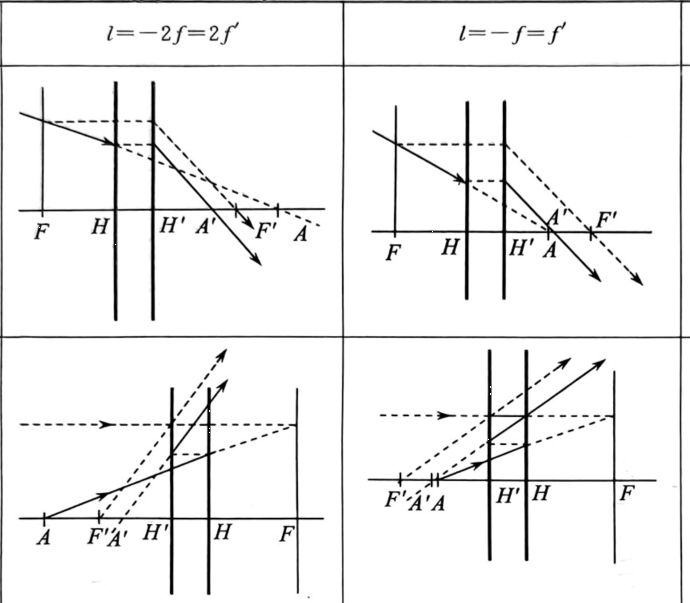
\includegraphics[width=8cm]{img/3.11.png}
        \end{figure}
\subsubsection{光束的汇聚度和系统的汇聚度}
首先直接给出几个概念
\begin{description}[nosep]% nosep没有垂直间隔
    \item[折合物距] $\displaystyle \frac{l}{n}$
    \item[折合像距]$\displaystyle \frac{l'}{n'}$
    \item[折合焦距]   $\displaystyle \frac{f'}{n'}$
    \item[汇聚度] $\displaystyle V=\frac{n}{l} \quad V'=\frac{n'}{l'}$,并且其为正代表光束是汇聚光束,反之为发散光束。
    \item[光焦度]  $\displaystyle \Phi'=\frac{n'}{f'}=\frac{-n}{f}$,正表示汇聚作用。表征光学系统偏折光线的能力。单位:屈光度——以米为单位的焦距的倒数。
\end{description}
\begin{equation}
\Phi=V'-V \tag{2.3.8}
\end{equation}
\subsubsection{透镜不同位置的成像情况}
        \begin{figure}[H]
            \centering
            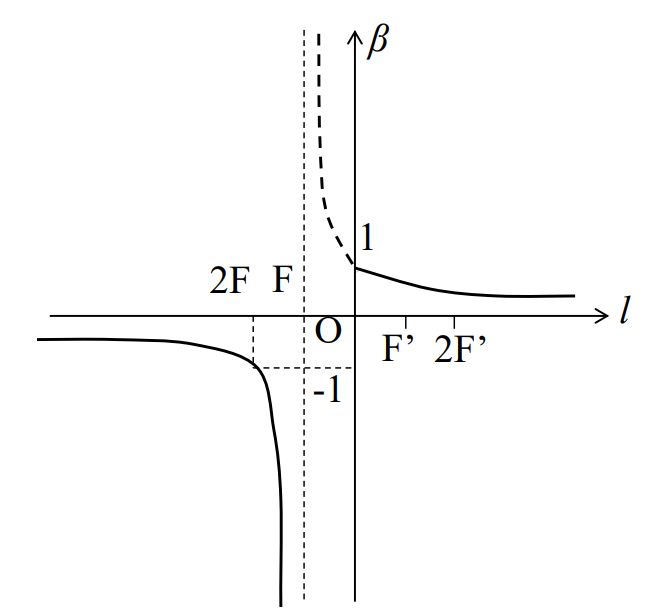
\includegraphics[width=8cm]{img/3.6.png}
            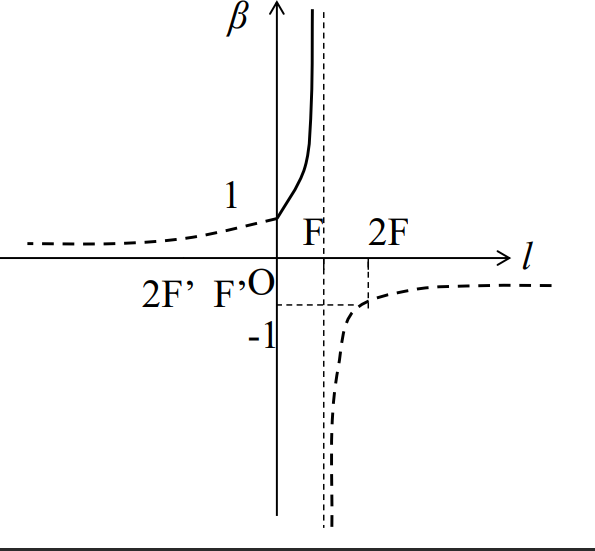
\includegraphics[width=8cm]{img/3.7.png}
            \caption[]{其实就看$when \quad l'=\infty$}
            上面的一个是正透镜,下面是负透镜。注意$F'$的位置。然后注意2F的位置是-1,原点是1,画出趋势图就行。
            $$
            \beta=\frac{nl'}{n'l}=-\frac{fl'}{f'l}
            $$
            \end{figure} 
\subsection{理想光学系统的组合分析}
\subsubsection{两个理想光学系统}
图解法,任意高度做一平行于光轴的线,经过光组在像方与入射线延长线相交。得到主面,另一方同理。(根据定义,主面高度相同)
        \begin{figure}[H]
            \centering
            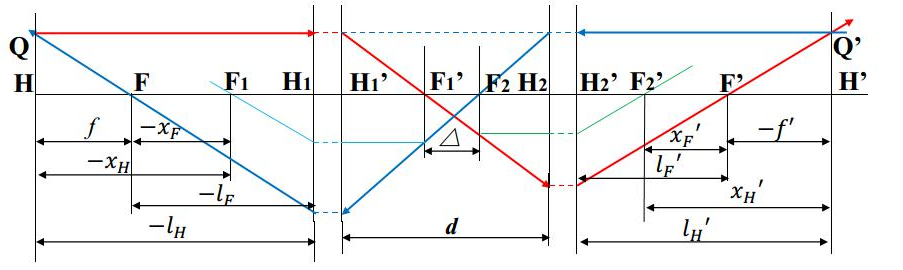
\includegraphics[width=8cm]{img/3.8.png}
            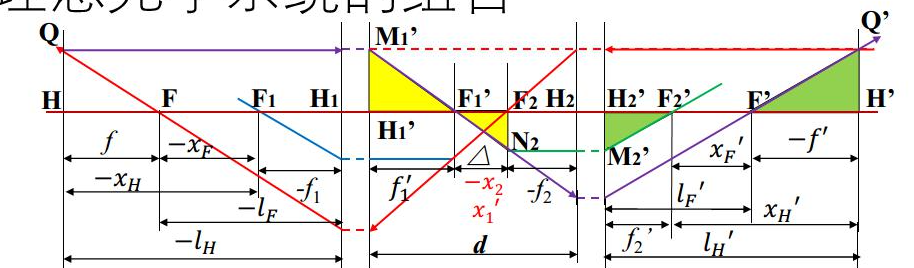
\includegraphics[width=8cm]{img/3.9.png}
        \end{figure}
然后我们对找完之后的图,来进行一下定量的分析。(以第二个光组的像方焦点、像方主点为起始点
——合成光组的物方参量 以第一个光组的物方焦点、物方主点为起始点。)直接列写
\begin{align}
    \Delta_i &=-f_i'+d+f'_{i+1} \tag{2.3.7.a} \\
     d_i&= H_i'H_{i+1}=l_i'-l_{i+1}\tag{2.3.7.b} \\
    \Delta_i&=F_i'F_{i+1}=f_i'-f_{i+1}\tag{2.3.7.c}
\end{align}
 
\subsubsection{像差和组合分析}
\section{平面与平面系统}
\section{光阑}
\begin{description}[leftmargin=1.7cm,style=nextline,nosep]% nosep没有垂直间隔
    \item[光阑 ]  光学系统中的一些中央开孔的挡光屏或光学元件的边缘。
    \item[孔径光阑    ] 限制成像光束口径的大小,
    \item[视场光阑    ] 限制成像范围的大小。
    \item[渐晕光阑
    ]遮挡轴外物体的部分光场,使像边缘模糊;

    
    \item[消杂光光阑    ]  消除镜面反射光、镜架炫光等引起的杂散光。

\end{description}
\subsection{入瞳出瞳和孔径角}
        \begin{figure}[H]
            \centering
            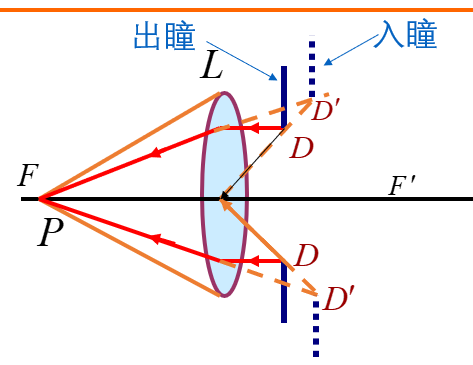
\includegraphics[width=8cm]{img/4.1.png}
            \end{figure}
入瞳是孔径光阑经过光阑后面的光学系统成的像,出瞳是经过前面的光学系统成的像。如果其在最前面,那本来就是入瞳,如果在最后面,本来就是出瞳。
\begin{description}[leftmargin=0.7cm,style=nextline,nosep]% nosep没有垂直间隔
    \item[物方孔径角] 轴上物点到入射光瞳 
\end{description}
\section{光学仪器}
\section{像差的种类和矫正}

\section{平面与平面系统}
\begin{definition}[平面光学元件]
    工作面为平面的光学元件,对物体没有放大和缩小的功能,分为平面折射和反射原件。
    \end{definition}
其可以
\begin{itemize}[nosep]
\item 改变光轴位置和方向
\item 改变像的坐标
\item 折叠光路,减小形体和质量
\item 分光
\item 测量,扩大系统观察范围
\end{itemize}
\subsection{平面镜}
平面反射镜,简称平面镜,\textbf{唯一成完善像元件}(理想成像)。
对于平面镜,常见性质为
\begin{align}
    r=\mathbf{-}\infty &\hspace{0.3cm}   n'=-n\tag{4.1.1.a}\\
    \beta=1& \hspace{0.3cm} l'=l \tag{4.1.1.b}\\
   y=y'& \tag{4.1.1.c}
\end{align}
\begin{description}[leftmargin=0.9cm,style=nextline,nosep]% nosep没有垂直间隔
    \item[镜像]  左右手坐标系颠倒。
    \item[$2\alpha$] 平面镜旋转$\alpha$,反射光线同方向旋转$2\alpha$
\end{description}
        \begin{figure}[H]
            \centering
            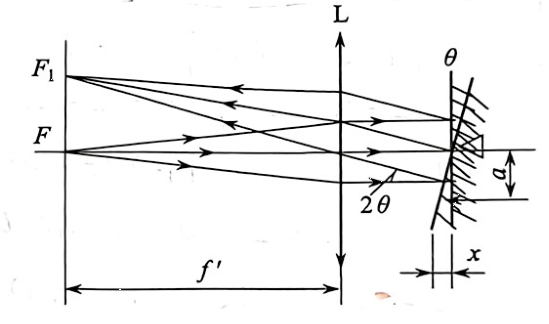
\includegraphics[width=7cm]{img/4.2.png}
            \end{figure}
$2\alpha$ 性质常被用于测量,如上图2所示,有
\begin{align}
    FF_1=2f'\theta \tag{4.1.2.a}\\
    FF_1=2f(\frac{a}{x}) \tag{4.1.2.b}
\end{align}
\subsubsection{双平面成像}
        \begin{figure}[H]
            \centering
            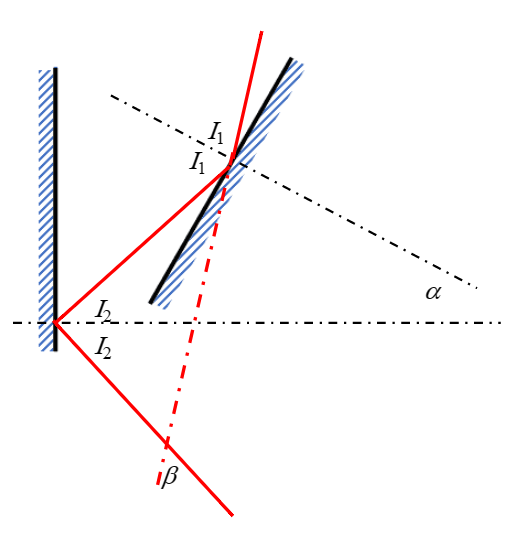
\includegraphics[width=5cm]{img/4.3.png}
            \end{figure}
出射光线与入射光线夹角只与平面镜二面角有关。设入射光线和出射光线单位向量分别为$\vec{r_{in}},\vec{r_{out}}$,第一个和第二个镜面单位法向量为(入射到的第一个)$\vec{n_1,\vec{v_2}}$。有
\begin{equation}
\frac{\cos <\vec{r_{in}},\vec{r_{out}}>}{\cos <\vec{n_1},\vec{n_2}>}=2\tag{4.1.3}
\end{equation}
\subsection{平行平板}
        \begin{figure}[H]
            \centering
            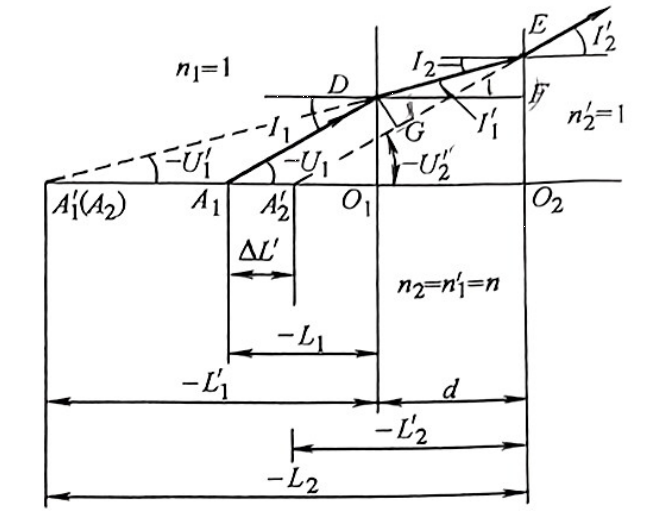
\includegraphics[width=6cm]{img/4.4.png}
        \end{figure}
\begin{equation}
\begin{aligned}
    \Delta T=DG&=\frac{DE}{\sin(I_1-I_1')} \\
    &=\frac{d}{\cos I_1'}\sin(I_1-I_1')\\
    &=\frac{d}{\cos I_1'}(\sin I_1\cos I_1'-\cos I_1\sin I_1')\\
    &=\frac{d}{\cos I_1'}[\sin I_1'(n \cos I_1'-\cos I_1)]\\
    &=d\sin I(1-\frac{\cos I_1}{n \cos I_1'})\\
    &=d\sin I(1-\frac{\tan I_1}{\tan I_1'})
    % &(n\sinI=n'\sinI')
\end{aligned}\tag{4.2.1}
\end{equation}

\begin{align}
\Delta L'&=\frac{DG}{\sin I_1} \tag{4.2.2.a}\\
&=d(1-\frac{\cos I_1}{n \cos I_1'})\tag{4.2.2.b}\\
&=d(1-\frac{\tan I_1}{\tan I_1'}) \tag{4.2.2.c}
\end{align}

显然,其不能成完善像。一些常见的符号含义
\begin{align}
    L_1=H_1A_1 &\hspace{0.3cm}   L_1'=H_1'A_1'\tag{4.2.3.a}\\
    L_2=H_1A_2 &\hspace{0.3cm}   L_2'=H_1'A_2'\tag{4.2.3.b}\\
   d=H_1H_1'& \hspace{0.3cm} \Delta L'=A_1 A_2' \tag{4.2.3.c}
\end{align}
显然
\begin{equation}
L_2'=-d+L_1+\Delta L'\tag{4.2.4}
\end{equation}
或者
\begin{equation}
\Delta L'=A_1A_2'=-L_1+d+L_2'\tag{4.2.5}
    \end{equation}

    \subsubsection{近轴区等效}
    \begin{equation}
    \Delta L'=d(1-\frac{1}{n}) \tag{4.2.6}
    \end{equation}
    等效空气平板
    \begin{equation}
    \overline{d}=d-\Delta L'=\frac{d}{n}\tag{4.2.7}
    \end{equation}
    轴向位移如下,换小写就行。
    \begin{quote}
    {\qquad\parindent2\ccwd\kaishu\zihao{5}
    所谓等效:
是指同一入射光线,在入射面的
投射高度相同,在出射面的投射
高度也相同;
    }
    \end{quote}
\subsection{反射棱镜}
\begin{description}[leftmargin=1.7cm,style=nextline,nosep]% nosep没有垂直间隔
    \item[光轴] 光学系统中的光轴在棱镜中的部分。
    \item[入射面和出射面] 
    \item[棱线] 工作面之间的郊交线  
    \item[主截面] 垂直于棱的截面  
    \item[光轴截面] 由光轴所决定的截面(和光轴重合)
    \item[简单棱镜] 只有一个主截面,并且所有工作面都和主截面垂直。按照反射面的类型可分为1,2,3。  
\end{description} 
\subsubsection{一次反射棱镜}直角,梯形,道威。
\begin{quote}
{\qquad\parindent2\ccwd\kaishu\zihao{5}
道威旋转$\alpha$,其成像旋转$2\alpha$。可以应用在周视旋转镜中,直角棱镜转速$\omega$,道威$\omega/2$,可以使得丞相不变。

}
\end{quote}
\subsubsection{二次反射棱镜} 主要说以下,屋脊棱镜。用交线位于棱镜光轴面内的两个互相垂直的反射
面代替棱镜的一个反射面,像转过180。
\subsubsection{三次反射棱镜}折叠光路,结构紧凑。

\subsubsection{棱镜成像方向的判定} 应该使用正像,不能是镜像或者倒。
\begin{itemize}[nosep]
\item $oz'$是出射光方向
\item 平行于主截面的$oy'$和屋脊棱镜有关,偶数相同,奇数相反。
\item 垂直于主截面的$ox'$看反射面(屋脊算2),偶数右手系,奇数左手系。注意它不是看正反,而是坐标系。
\end{itemize}

对于多个主截面的话,依次分析。
\subsection{折射棱镜}
\subsubsection{偏向角}
\begin{equation}
    \sin \frac{\alpha + \delta}{2}= \frac{n \sin \frac{a}{2}\cos \frac{1}{2}(I_{1}^{\prime}+I_{2})}{\cos \frac{1}{2}(I_{1}+I^{\prime}_{2})} \tag{4.4.1}
\end{equation}
当$ I_{1}+I_{2}^{\prime}=0,I_{1}^{\prime}-I_{2}=0 $时,偏向角δ有最小值 $  \delta _{m} $,满足公式
\begin{equation}
    \sin \frac{\alpha + \delta _{m}}{2}=n \sin \frac{\alpha}{2} \tag{4.4.2}
\end{equation}
\subsection{光楔}
光楔
\begin{equation}
    \delta = \delta _ { 1 } - \delta _ { 2 }=( n - 1 ) \alpha \tag{4.4.3}
\end{equation}

色散

\begin{quote}
{\parindent2\ccwd\kaishu\zihao{5}
同一种透明介质对不同波长的色光具有不同的折射率。由于介质的不同,其折射率随波长的变化程度不同,这种性质称为色散
}
\end{quote}

色散系数如下
\begin{equation}
    n=A+ \frac{B}{\lambda ^{2}}+ \frac{C}{\lambda ^{4}} \tag{4.4.5}
\end{equation}
红光波长最长,之后递减。所以$n$ 递增,偏角递增,偏向下。
\section{光阑}
\begin{description}[leftmargin=1.7cm,style=nextline,nosep]% nosep没有垂直间隔
    \item[光阑 ]  光学系统中的一些中央开孔的挡光屏或光学元件的边缘。
    \item[孔径光阑    ] 限制成像光束口径的大小,
    \item[视场光阑    ] 限制成像范围的大小。
    \item[渐晕光阑
    ]遮挡轴外物体的部分光场,使像边缘模糊;

    
    \item[消杂光光阑    ]  消除镜面反射光、镜架炫光等引起的杂散光。

\end{description}
\subsection{入瞳出瞳和孔径角}
        \begin{figure}[H]
            \centering
            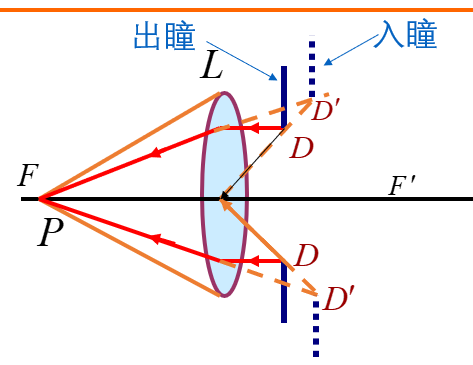
\includegraphics[width=8cm]{img/4.1.png}
            \end{figure}
入瞳是孔径光阑经过光阑后面的光学系统成的像,出瞳是经过前面的光学系统成的像。如果其在最前面,那本来就是入瞳,如果在最后面,本来就是出瞳。
\begin{description}[leftmargin=0.7cm,style=nextline,nosep]% nosep没有垂直间隔
    \item[物方孔径角] 轴上物点到入射光瞳 
\end{description}
\section{光学仪器}
\subsection{人眼}
\begin{itemize}
\item 
可见光的波长范围从400-760nm,人眼最灵敏的光波长为550nm。
\item  人眼瞳孔为\textbf{孔径光阑}
\end{itemize}
\begin{quote}
{\qquad\parindent2\ccwd\kaishu\zihao{5}
光照充足时对550nm最敏感;光照弱时对510nm敏感。
}
\end{quote}
\subsubsection{人眼的自动调节}
\begin{figure}[H]
    \centering
    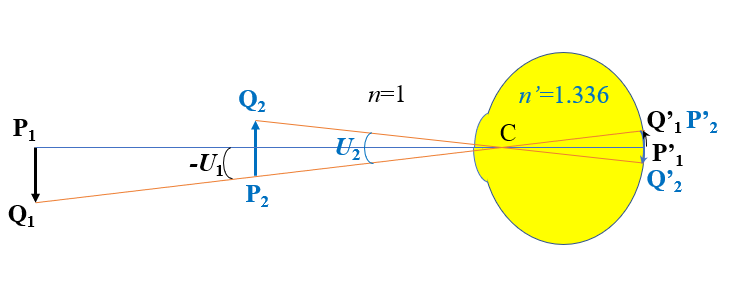
\includegraphics[width=7cm]{img/5.1.png}
    \end{figure}
\begin{description}[leftmargin=1.7cm,style=nextline,nosep]% nosep没有垂直间隔
    \item[远点] 眼睛调节到最远的距离,此时晶状体最薄,肌肉最松弛。
    \item[近点]   眼睛调节到最近的距离,此时晶状体最厚,肌肉最紧张。
    \item[远点距 r]  远点到眼睛物方主点的距离,注意$<0$
    \item[近点距 p ] ...
    \item[屈光度]  $R=1 /r ,P=1 /p ,A=R-P$
    \item[明视距离] $250mm$ 
    \item[视角]  人眼对物体的张角,遵从符号规则。 

\end{description}
\begin{equation}
\frac{1}{l_r}-\frac{1}{l_p}=R-P=A
\end{equation}

\subsubsection{非正常眼及其矫正}
        \begin{figure}[H]
            \centering
            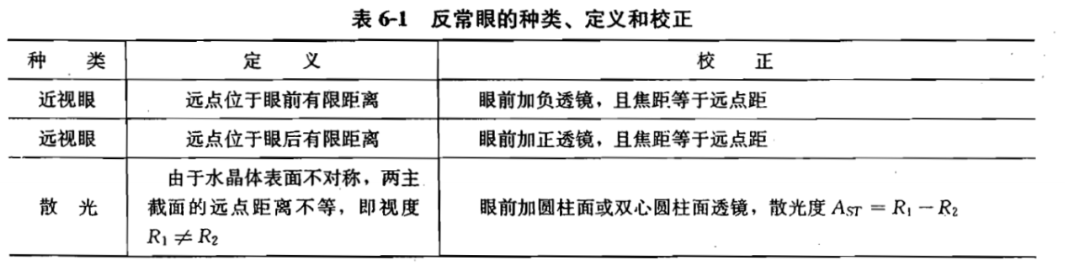
\includegraphics[width=7cm]{img/5.3.png}
            \end{figure}
\begin{quote}
{\qquad\parindent2\ccwd\kaishu\zihao{5}
1D 等于100 光焦度。对于正常眼,有$r=\infty,R=0,F'$ 在视网膜上。
}
\end{quote}
\begin{align*}
\Phi=\frac{1}{f'}=\frac{1}{l'}-\frac{1}{l}    
\end{align*}
对于所带光学系统而言,$l'=0.25$,l代入远点距。其实就是把无穷远处或者明视范围的物体成像到远点上。
\subsubsection{眼睛的自适应}
\begin{quote}
{\qquad\parindent2\ccwd\kaishu\zihao{5}
瞳孔直径改变
2~8mm

}
\end{quote}
\subsubsection{分辨本领}[]
\begin{definition}[极限分辨角]
    最靠近二点对人眼(物方节点)的张角$\phi$
\end{definition}
\begin{equation}
\phi=\frac{1.22 \lambda}{D(\text{入瞳直径})}\tag{6.1.2}
\end{equation}
一般取1度。

\section{放大镜}
视觉放大倍率,用\textbf{厘米}为单位。
\begin{equation}
    \Gamma =y_{i}^{\prime}/y_{e}^{\prime}=(l^{\prime}\tan \omega ^{\prime})/(l^{\prime}\tan \omega)= \tan \omega ^{\prime}/ \tan \omega  \tag{6.1.3}
\end{equation}

        \begin{figure}[H]
            \centering
            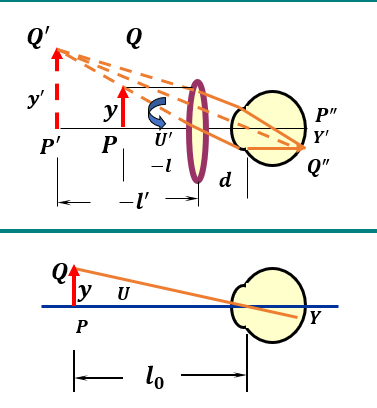
\includegraphics[width=7cm]{img/6.1.png}
            \end{figure}
\begin{equation}
\begin{aligned}
M_1&=\frac{\tan U'}{\tan U}=\frac{1}{\frac{y}{l_0}} \frac{y'}{-l'+d} \\
&=\frac{l_0}{y}\frac{y'}{d-l'}=\beta \frac{l_0}{d-l'}\\
&= \frac{l_0}{d-l'} -\frac{x'}{f'}=\frac{l_0}{f'} \frac{l'-f'}{l'-d} 
\end{aligned} \tag{6.1.4}
\end{equation}
$l'=-\infty$适合长时间观察,眼睛最放松.视角放大率与放大镜到眼睛距离无关.

如果在明视距离处,有
\begin{align}
   d-l'&=l_0 \tag{6.1.5.a}\\
   M&=-\frac{l'-f'}{f'}=\Phi  \tag{6.1.5.b} \\
   M&=\frac{f'-(d-l_0)}{f'}=\frac{l_0}{f'}+1-\frac{d}{f'} \tag{6.1.5.c}
\end{align}
当$d\to 0$ 
\begin{equation}
M_2=\frac{l_0}{f'}+1 \thickapprox M_2 \tag{6.1.6}
\end{equation}

\subsection{显微镜}
\begin{quote}
{\qquad\parindent2\ccwd\kaishu\zihao{5}
目:eye 物:obj。小物位于物镜焦点外侧,中间放大实像在$L_e$ 的物方焦面上,最后生成无限远或者明视距离放大的虚像。
}
\end{quote}
        \begin{figure}[H]
            \centering
            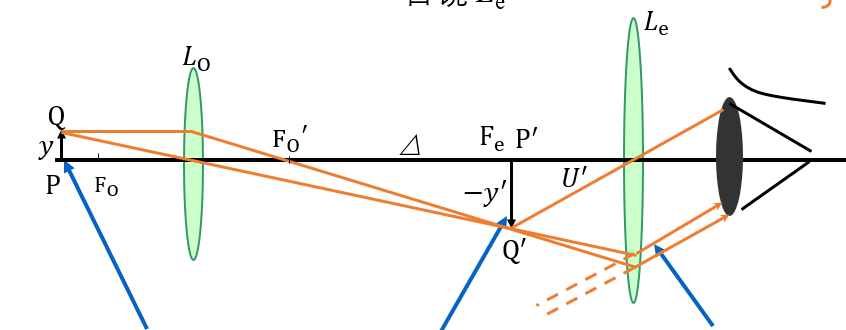
\includegraphics[width=8cm]{img/6.2.png}
            \caption*{注意看它的变量的表示}
            \end{figure}
最显然的,我们有
\begin{align}
    \Delta&=F'oF_e \tag{6.2.1.a} \\
     \tan U&=\frac{y}{l_0} \tag{6.2.1.b} \\
     \tan U'&=\frac{-y'}{f'_e}=--\frac{y'}{f'_e}=\frac{y'}{f'_e} \tag{6.2.1.c} \\
     M&=\frac{\tan U' }{\tan U}=\frac{l_0}{y}\frac{y'}{f'_e}=\beta_o M_e\tag{6.2.1.d}\\
     \beta_0&=-\frac{\Delta}{f_o'}\tag{6.2.1.e}\\     
     M&=-\frac{\Delta l_0}{f_o'f_e'}=\frac{l_0}{f'}\tag{6.2.1.f}
\end{align}
\subsection{望远镜}
        \begin{figure}[H]
            \centering
            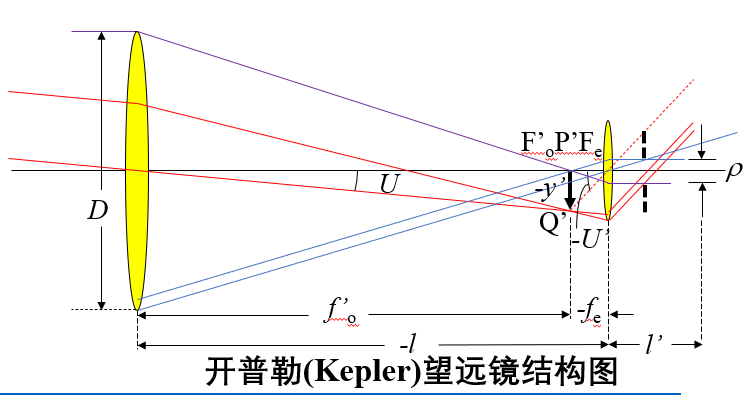
\includegraphics[width=8cm]{img/6.3.png}
            \end{figure}

\begin{quote}
{\qquad\parindent2\ccwd\kaishu\zihao{5}
观察无限远物体(天体)时望远镜的光学间隔为零,
观察有限远景物时望远镜的光学间隔很小。

}
\end{quote}
        \begin{figure}[H]
            \centering
            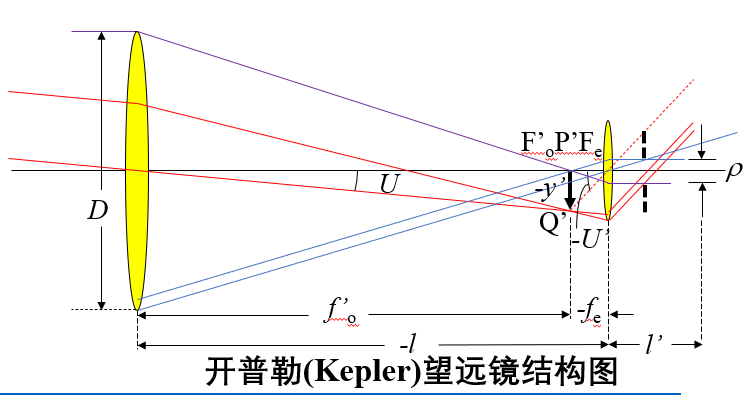
\includegraphics[width=7cm]{img/6.3.png}
            \end{figure}
该物体直接对眼镜成的像是
\begin{align}
\tan U&=\frac{-y'}{f'_o} \tag{6.3.1.a}\\
\tan -U'&=\frac{-y'}{-f'_e} \tag{6.3.1.b}\\
M&=\frac{\tan U'}{\tan U}=-\frac{f'_o}{f'_e}=-\frac{D}{\rho} \tag{6.3.1.c}
\end{align}
\begin{figure}[H]
    \centering
    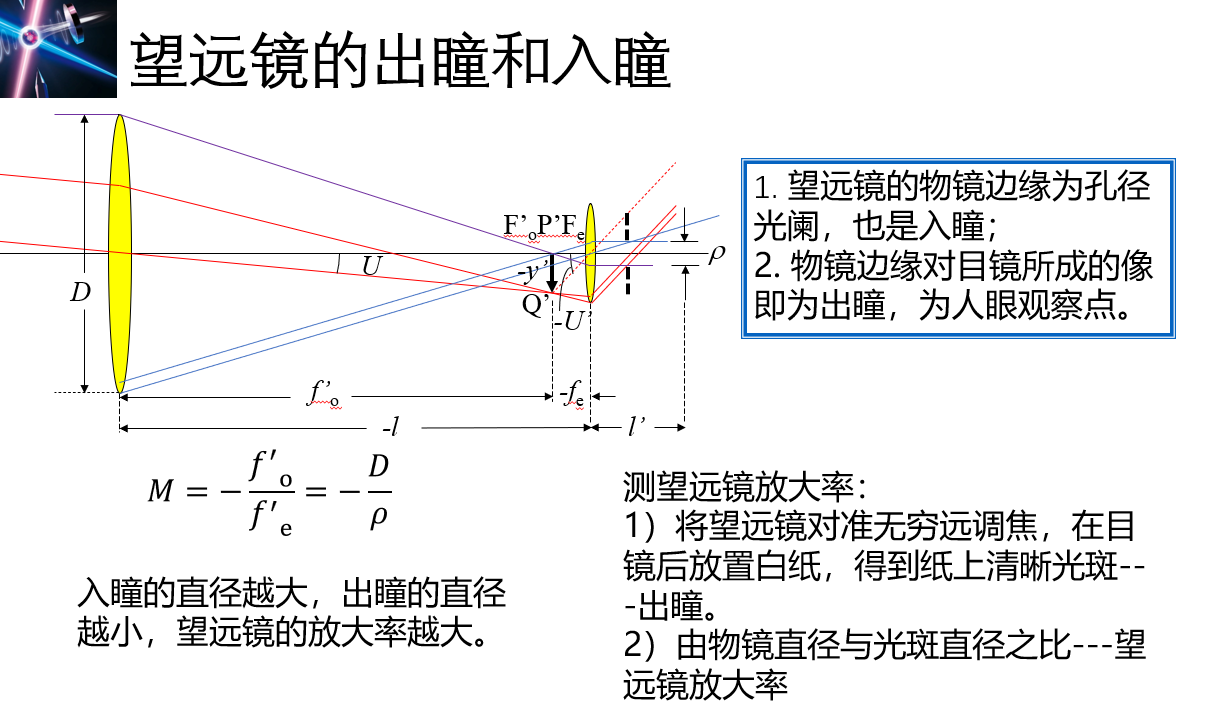
\includegraphics[width=7cm]{img/6.5.png}
    \end{figure}
\subsection{目镜}
目镜分为惠更斯(Huygens)目镜和冉斯登(Ramsten)目镜。
\subsection{照相机}
\subsection{投影仪}
\section{像差的种类和矫正}
        \begin{figure}[H]
            \centering
            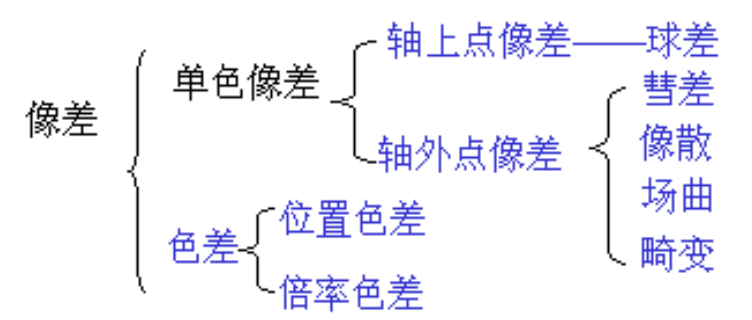
\includegraphics[width=7cm]{img/6.6.png}
            \end{figure}
\subsection{球差及其矫正}
球差是$\delta L=L'-l'$,正就是正球差,负就是负数球差。轴上,
\subsection{齐明点}
\begin{equation}
     nL=n'L=(n+n')r \tag{6.7.1}
\end{equation}
\begin{equation}
\beta=\frac{nL'}{n'L} \tag{6.7.2}
\end{equation}
三对齐明点另外的是
\begin{align}
 L&=L'=r \tag{6.7.3.a}\\
 L&=0   
\end{align}
\begin{quote}
{\qquad\parindent2\ccwd\kaishu\zihao{5}
注意上面的是像物距。
}
\subsubsection{等光程}
\end{quote}
\section{题目}
\begin{itemize}
\item 光程等于\textbf{介质中传播的几何路程何其折射率}的乘积
\item 基面一般是指(                    \textbf{ 焦平面、主平面和节平面}
)
理想光学系统不可能获得与立体物体相似的立体像是因为      ( \textbf{立体物体的轴向放大率和垂轴放大率是不等的
})
\item 注意明视距离         \begin{figure}[H]
            \centering
            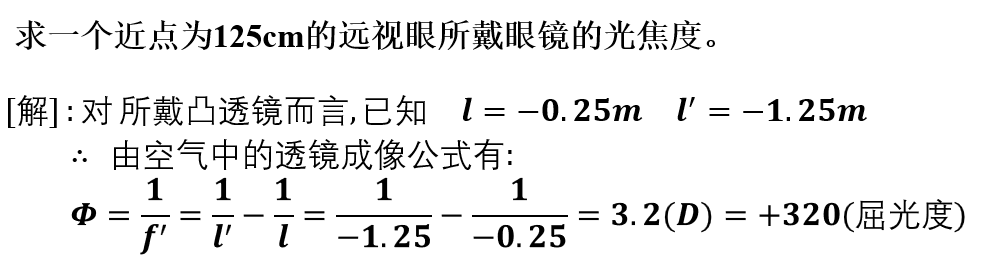
\includegraphics[width=8cm]{img/t1.png}
            \end{figure}
\end{itemize}

\end{document}